\subsubsection{Visualizing phase diagrams}
\label{sec:visualizing-phase-diagram}
\textit{This section was contributed by Haoyuan Li and Magali Billen.}

For many models it is useful to see how the material parameters vary as a function of pressure and temperature. In this cookbook, a plot of material properties (e.g., density or viscosity) as a function of temperature (x axis) and pressure (y axis) is referred to as a phase diagram. 

In this phase diagram cookbook, phase diagrams are generated from model runs and visualized with VisIt, but ParaView could also be used to view the same output. % intro
This is a simple way of using the visualization output to check the correct implementation of phase transitions in a material model. 
The idea lies in using a model with an initial temperature that increases linearly along the $x$-axis and a pressure that changes linearly along the $y$-axis in a box geometry, so that the two axes, $x$ and $y$, can be interpreted as axes for pressure and temperature in the graphical output. 
Here, we visualize a diagram of the phase transitions implemented in the visco plastic material model, as well as a lookup table in the Steinberger material model. 

\paragraph{The input file.}
You can find the input file to run this cookbook example in \url{cookbooks/visualizing_phase_diagram/visualizing_phase_diagram.prm}. For this first case, phase transitions are prescribed manually in terms of their depth, Clapeyron slope, and other key parameters. 

The model domain is  800 km  by 800 km box. % geometry
Initial temperature increases from \SI{273}{K} on the left side to \SI{2273}{K} on the right side. % initial conditions
Pressure, on the other hand, increases from the top of the box to the bottom with a constant gradient.
This is assured by assigning a constant density with zero expansivity.
It differs from a classic phase diagram only in the direction of pressure increase.

Two compositions of pyrolite and harzburgite are included in the model. % composition
With each run, only one composition is assigned to the whole domain in order to visualize the diagrams of these two separately.

The material model is then set up to mimic mantle phase transitions at 410, 520, and \SI{660}{km}. % setup of mantle transitions
Details of phase transitions are taken from \cite{billen2018decoupling}.
A trick is needed to make this work: we assign the values of the density to the field of heat capacity in the input file. % trick
To do this, We use the phase inputs implemented in the visco plastic plug-in.
This serves the goal of visualizing values of reference densities of phases with the real density assigned with a constant value in the model.
Inputs for this material model are listed here:
\lstinputlisting[language=prmfile]{cookbooks/visualizing_phase_diagram/doc/material_model.prm.out}


\paragraph{Results.}

Visualization of the model results yields a phase diagram of a pyrolitic mantle (Figure \ref{fig:phase_diagram_ph_density}). % phase diagram
The field shown here has the reference densities of the pyrolite phases, though settings of phase transitions are over-simplified.
One may notice that three transitions (i.e., one in the olivine system, two in the spinel system) are included for the 660 interfaces, % 3 transitons, higher T
and they need to be modified at a higher temperature.
In spite of the complexities of mantle phases, the focus of this first example is to simply illustrate this approach of visualizing it.
Beyond showing the diagram, We have also used the ``lineout'' feature in VisIt to export the data along two vertical lines at $T = \SI{1173}{K}$ and $T = \SI{1673}{K}$ (Figure \ref{fig:phase_diagram_ph_profile}). % linear profile
The figure for $T = \SI{1173}{K}$ illustrates the buoyancy forces felt by a descending cold slab within the mantle transition zone.

Next, we shift to harzburgite by changing the values of the initial compositional field from 0 to 1.  % harzburgite
For this to occur, the following changes are needed:
\lstinputlisting[language=prmfile]{cookbooks/visualizing_phase_diagram/doc/harzburgite.prm.out}
With this change, we can also visualize the phase diagram of harzburgite in Figure \ref{fig:phase_diagram_ph_density}.

Moreover, We tested the pyrolitic lookup table used in the Steinberg material model (Figure \ref{fig:phase_diagram_steinberg_density}).% steinberg model
The same setup of the initial condition is applied as in the previous case. % initial condition
The densities, however, are not assigned to the heat capacity anymore.
Thus the vertical axis would deviate from the axis of pressure a little bit.
This second setup serves the goal of illustrating a more complex and thus more realistic model of phase transitions.
Modification for the material model is listed below:
\lstinputlisting[language=prmfile]{cookbooks/visualizing_phase_diagram/doc/steinberg.prm.out}  % add 

Compared to the first example, pyrolitic phases are illustrated on a much finer scale.  % comparison 
Meanwhile, we can still tell the phase transitions at 410, 520, and $\SI{660}{km}$ depth, respectively, marked by linear boundaries analogous to a constant Clapeyron slope.


%%%%% figures %%%%%%
%%%%%%%%% figures1: pyrolite %%%%%%
\begin{figure}
\phantom.
\hfill
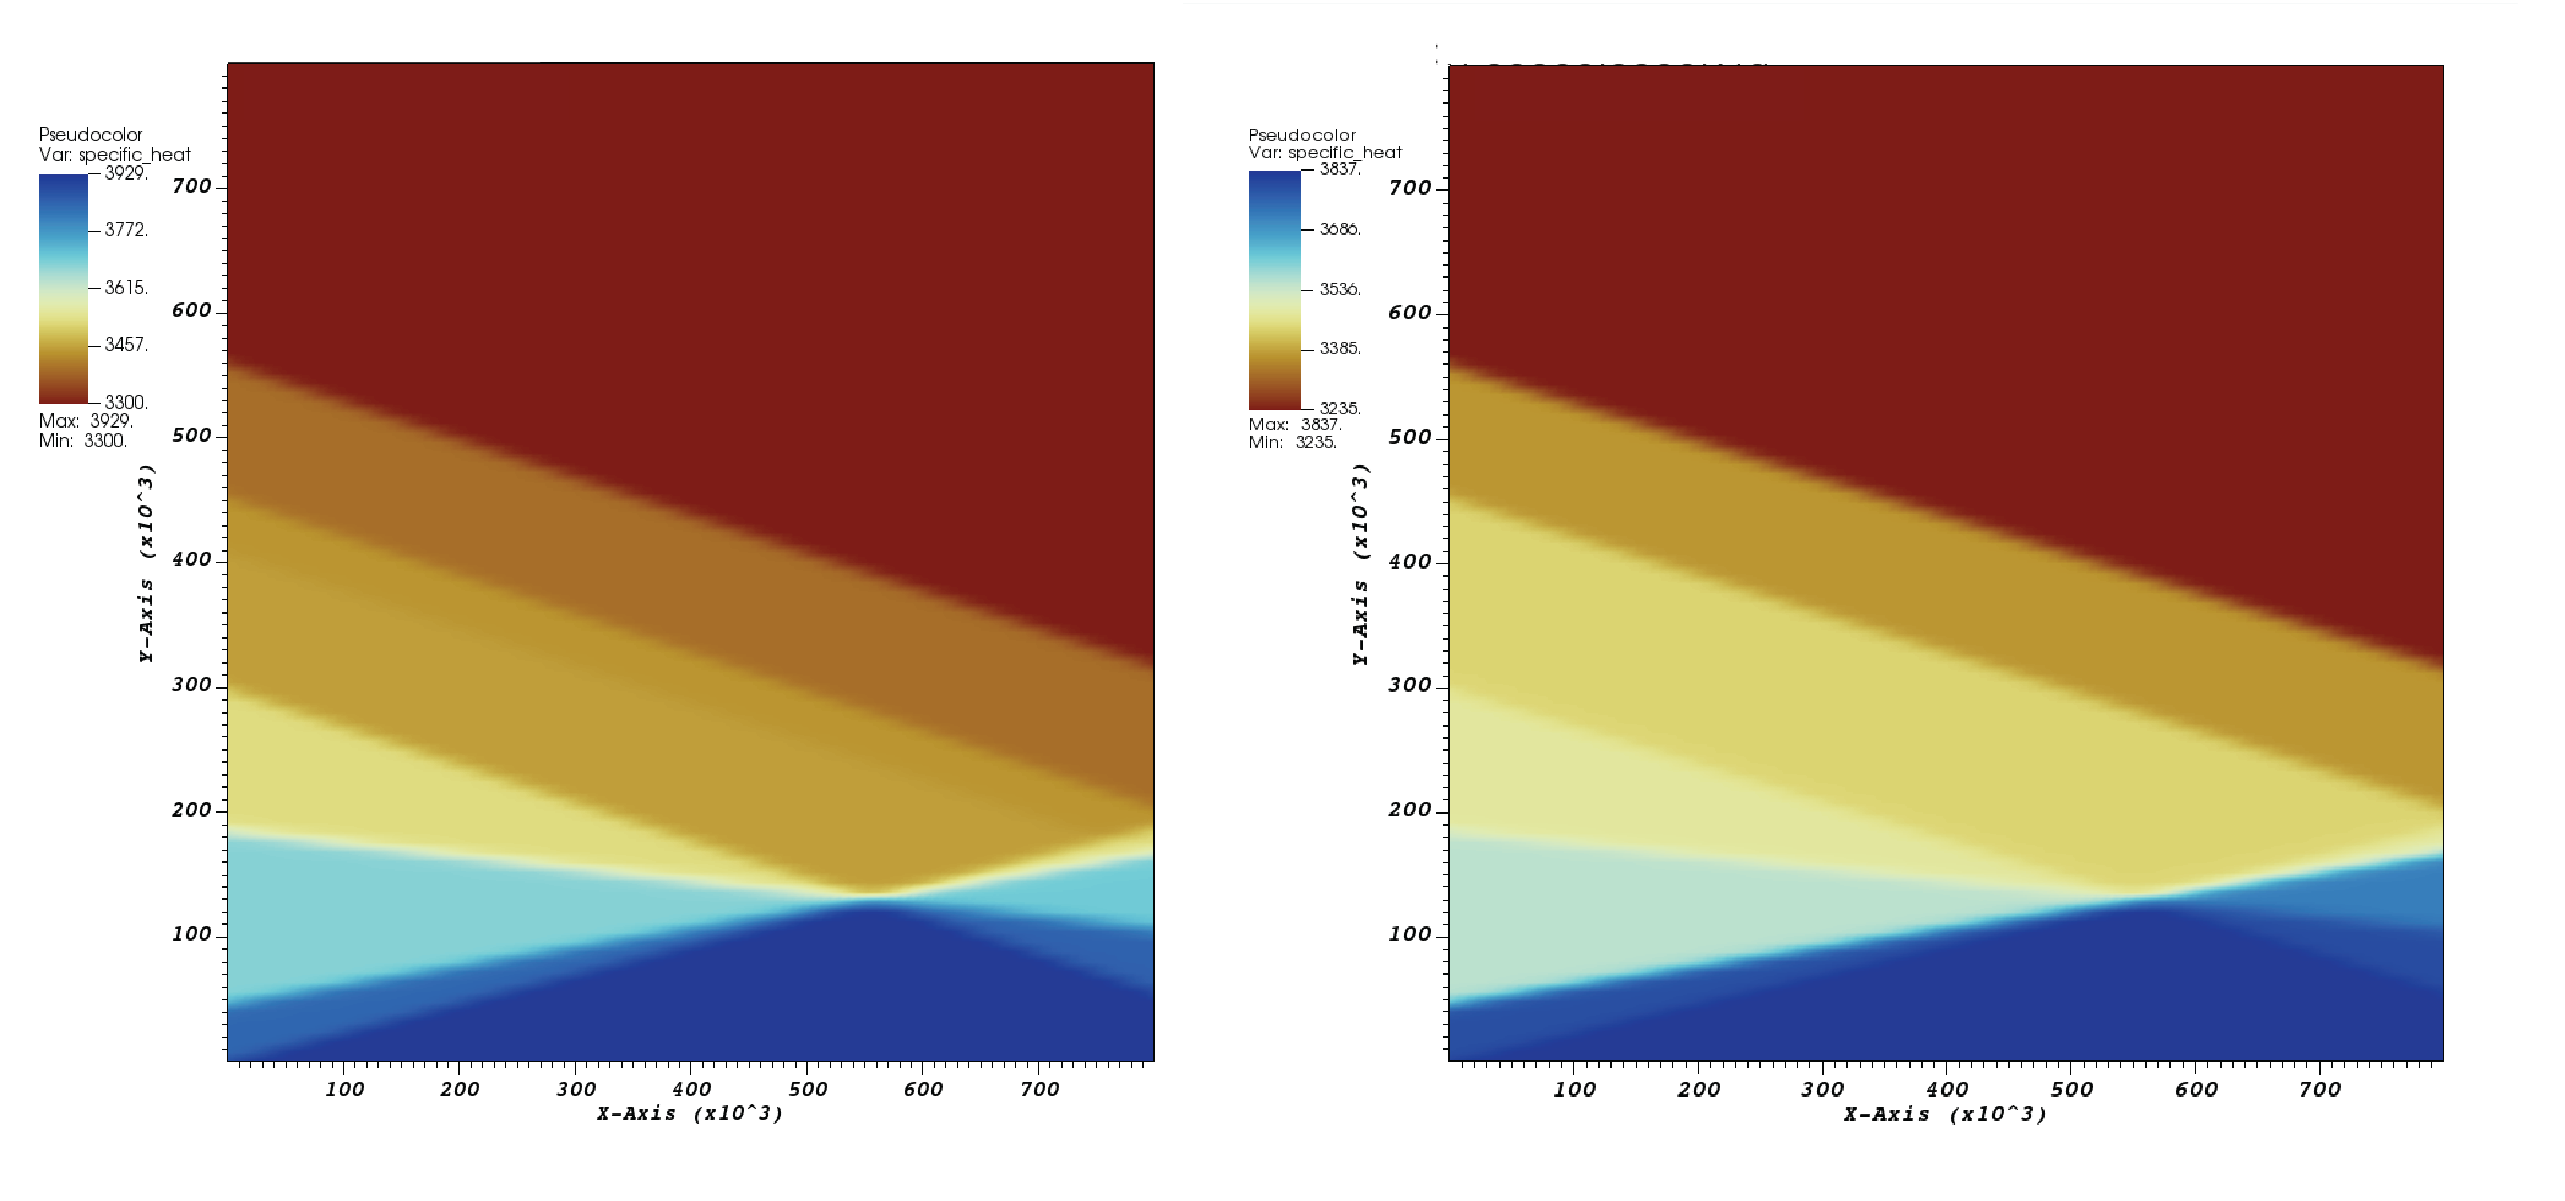
\includegraphics[width=0.9\textwidth]{cookbooks/visualizing_phase_diagram/doc/pyrolite_harzburgite.png}
\hfill
\phantom.
\caption{\it Visualization of phase diagrams: The field of heat capacity showing values of reference densities for pyrolitic and harzburgitic phases.}
\label{fig:phase_diagram_ph_density}
\end{figure}

%%%%%%%%%% figures2: pyrolite profiles %%%%%%
\begin{figure}
\centering
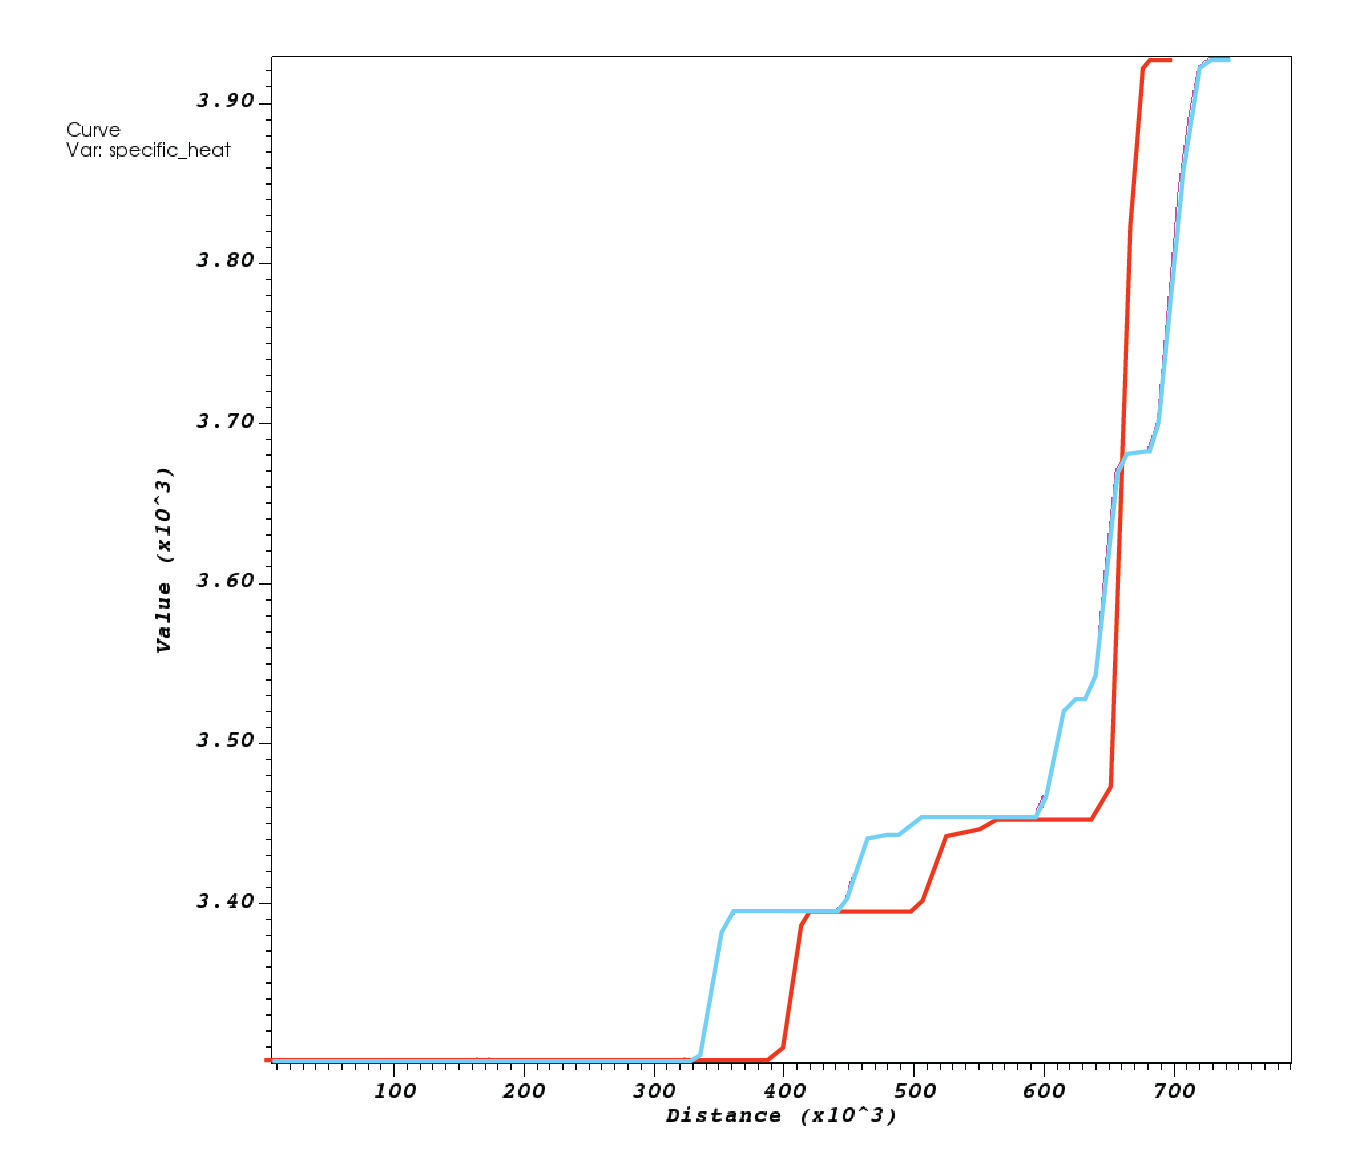
\includegraphics[width=0.4\textwidth]{cookbooks/visualizing_phase_diagram/doc/pyrolite_linear.png}
\caption{\it Visualization of phase diagrams: Profiles of pyrolitic density at $T=\SI{1173}{K}$ (red) and $\SI{1673}{K}$ (blue).}
\label{fig:phase_diagram_ph_profile}
\end{figure}
%%%%%%%%% figures3: lookup table %%%%%%
\begin{figure}
\centering
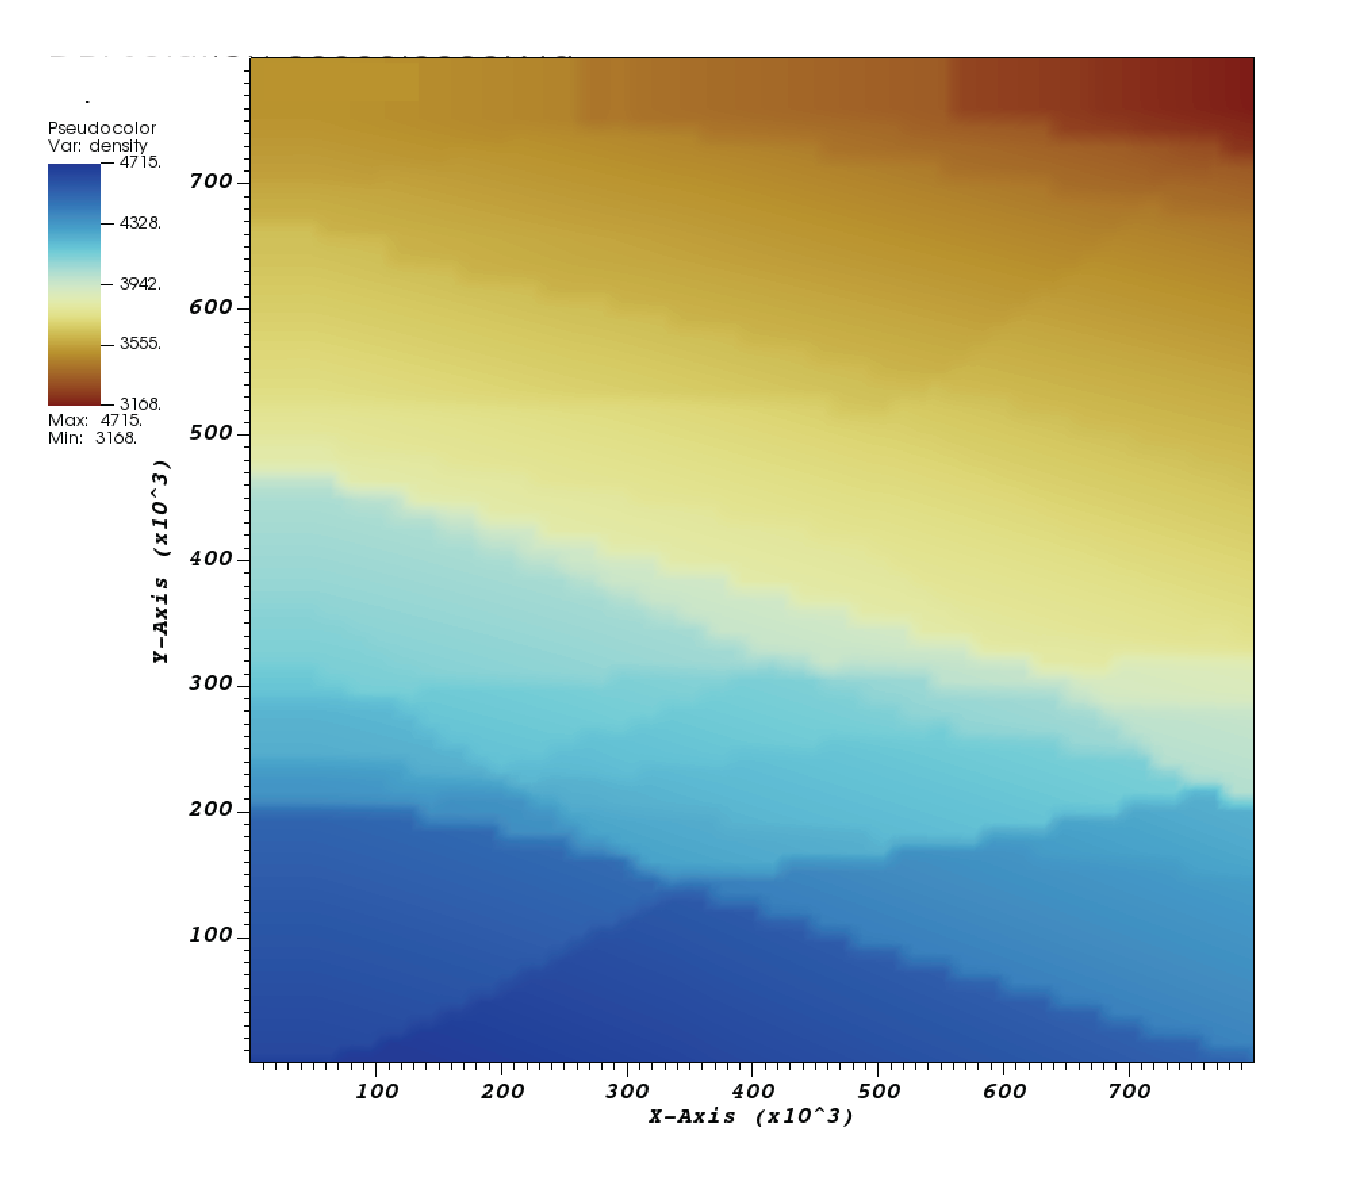
\includegraphics[width=0.4\textwidth]{cookbooks/visualizing_phase_diagram/doc/steinberg.png}
\caption{\it Visualization of phase diagrams: Density from lookup table of pyrolite from \cite{stixrude2011thermodynamics}.} % cite
\label{fig:phase_diagram_steinberg_density}
\end{figure}
